\documentclass[border=6pt]{standalone}
\usepackage{amsmath,amssymb}
\usepackage{pgfplots}
\pgfplotsset{compat=1.17}
\usepgfplotslibrary{fillbetween}
\definecolor{arcA}{RGB}{31,94,165}\definecolor{arcC}{RGB}{214,96,33}\definecolor{band}{RGB}{200,214,232}
\begin{document}
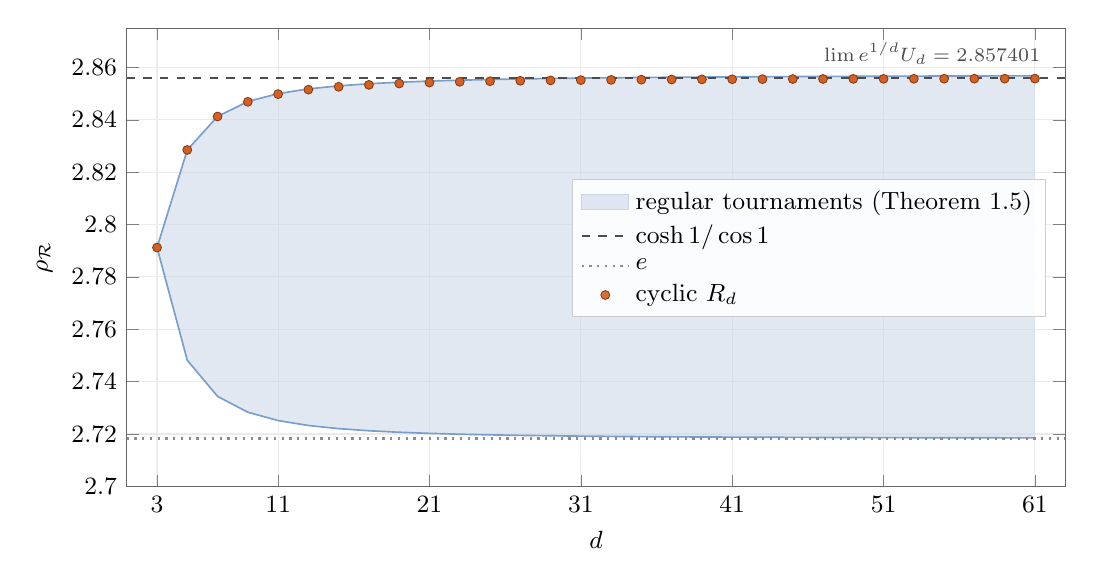
\begin{tikzpicture}
\begin{axis}[width=13.5cm,height=7.4cm,xmin=1,xmax=63,ymin=2.70,ymax=2.875,
  xlabel={$d$},ylabel={$\rho_{\mathcal R}$},xtick={3,11,21,31,41,51,61},
  ytick={2.70,2.72,2.74,2.76,2.78,2.80,2.82,2.84,2.86},yticklabel style={/pgf/number format/fixed,/pgf/number format/precision=2},
  tick label style={font=\small},label style={font=\small},axis line style={black!60},
  grid=major,grid style={black!8},legend style={font=\small,draw=black!20,fill=white,fill opacity=0.9,text opacity=1,at={(0.98,0.52)},anchor=east},
  legend cell align=left]
\addplot[name path=up,draw=arcA!60,line width=0.6pt] coordinates {(3,2.791225) (5,2.828512) (7,2.841306) (9,2.847000) (11,2.850021) (13,2.851823) (15,2.852991) (17,2.853795) (19,2.854376) (21,2.854811) (23,2.855147) (25,2.855413) (27,2.855627) (29,2.855803) (31,2.855950) (33,2.856073) (35,2.856179) (37,2.856271) (39,2.856350) (41,2.856420) (43,2.856481) (45,2.856536) (47,2.856585) (49,2.856629) (51,2.856668) (53,2.856704) (55,2.856737) (57,2.856767) (59,2.856794) (61,2.856820)};
\addplot[name path=low,draw=arcA!60,line width=0.6pt] coordinates {(3,2.791225) (5,2.748156) (7,2.734376) (9,2.728318) (11,2.725132) (13,2.723253) (15,2.722053) (17,2.721240) (19,2.720665) (21,2.720242) (23,2.719923) (25,2.719675) (27,2.719480) (29,2.719323) (31,2.719195) (33,2.719089) (35,2.719001) (37,2.718926) (39,2.718863) (41,2.718808) (43,2.718761) (45,2.718720) (47,2.718683) (49,2.718652) (51,2.718623) (53,2.718598) (55,2.718576) (57,2.718556) (59,2.718538) (61,2.718521)};
\addplot[band,fill opacity=0.55] fill between[of=up and low];
\addplot[black!70,dashed,line width=0.7pt,domain=1:63,samples=2] {2.8559578926};
\addplot[black!45,dotted,line width=0.8pt,domain=1:63,samples=2] {2.7182818285};
\addplot[only marks,mark=*,mark size=1.6pt,arcC,mark options={draw=arcC!60!black,line width=0.3pt}] coordinates {(3,2.791225) (5,2.828512) (7,2.841275) (9,2.846896) (11,2.849829) (13,2.851543) (15,2.852630) (17,2.853360) (19,2.853874) (21,2.854250) (23,2.854533) (25,2.854751) (27,2.854922) (29,2.855060) (31,2.855172) (33,2.855264) (35,2.855341) (37,2.855406) (39,2.855461) (41,2.855508) (43,2.855549) (45,2.855584) (47,2.855615) (49,2.855643) (51,2.855667) (53,2.855688) (55,2.855708) (57,2.855725) (59,2.855740) (61,2.855754)};
\legend{,,regular tournaments (Theorem 1.5),$\cosh 1/\cos 1$,$e$,cyclic $R_d$}
\node[font=\scriptsize,anchor=south east,black!70] at (axis cs:62,2.8575) {$\lim e^{1/d}U_d=2.857401$};
\end{axis}
\end{tikzpicture}
\end{document}
